%\usepackage[russian]{babel}
%\usepackage{graphicx}
%\usepackage{amsfonts}
%\usepackage{amssymb}
%\usepackage{amsmath}
%  ]{geometry}
%\usepackage[cp1251]{inputenc}
%\usepackage[english,russian]{babel}
%\usepackage{indentfirst}
%\graphicspath{{fig/}}
% --------------------------------------------------------------------------


\documentclass[aps,preprint,showkeys,
]{revtex4}
\usepackage{eurosym}
\usepackage{graphicx}
\usepackage{amsfonts}
\usepackage{amssymb}
\usepackage{amsmath}
\usepackage{epsfig}
\usepackage{color}

\newcommand{\la}{\langle}
\newcommand{\ra}{\rangle}

\begin{document}

\title{Localized modes in the Gross-Pitaevskii equation with a parabolic
trapping potential and a nonlinear lattice pseudopotential}
\author{G. L. Alfimov$^{1}$}
\author{L. A. Gegel$^{1}$}
\author{M. E. Lebedev$^{1}$}
\author{Boris A. Malomed$^{2,3}$}
\author{D. A. Zezyulin$^{3,4}$}
\affiliation{$^{1}$Moscow Institute of Electronic Engineering, Zelenograd, Moscow,
124498, Russia.}
\affiliation{$^{2}$Department of Physical Electronics, School of Electrical Engineering,
Faculty of Engineering, Tel Aviv University, Tel Aviv 69978, Israel}
\affiliation{$^{3}$ITMO University, St.~Petersburg 197101, Russia}
\affiliation{$^{4}$Institute of Mathematics with Computer Center, Ufa Scientific Center,
Russian Academy of Sciences, Chernyshevskii str., 112, Ufa 450008, Russia}

\begin{abstract}
We study localized modes (LMs) of the one-dimensional
Gross-Pitaevskii/nonlinear Schr\"{o}dinger equation with a
harmonic-oscillator (parabolic) confining potential, %$V(x)$
and a periodically modulated coefficient in front of the cubic term
(nonlinear lattice pseudopotential). The equation applies to a cigar-shaped
Bose-Einstein condensate loaded in the combination of a magnetic trap and an
optical lattice which induces the periodic pseudopotential via the Feshbach
resonance. Families of stable LMs in the model feature specific properties
which result from the interplay between spatial scales introduced by the
parabolic trap and the period of the nonlinear pseudopotential. Asymptotic
results are also obtained in the case of a rapidly oscillating nonlinear
pseudopotential. We show that the presence of the lattice pseudopotential
may result in: (i) creation of new LM families which have no counterparts in
the case of the uniform nonlinearity; (ii) stabilization of some previously
unstable LM species; (iii) evolution of unstable LMs into a breather trapped
in one well of the lattice pseudopotential.
\end{abstract}

\keywords{collisionally inhomogeneous BEC}
\date{\today}
\maketitle

%\date{\date{\today}}
%\documentclass{article}
%\usepackage[utf8]{inputenc}
%\usepackage[T2A]{fontenc}
%\usepackage[english, russian]{babel}
%\usepackage{graphicx}
%\usepackage{subcaption}
%\usepackage{float}
%\usepackage{amssymb,amsmath}

\graphicspath{ {images/} } %\begin{document}

\section{Introduction}

Since the first production of the Bose-Einstein condensate (BEC) in
ultracold gases \cite{AEMWC95,DMADDKK95,BSTH95}, great progress has been
made in the experimental work with BEC, leading to the observation of
diverse species of matter waves, such as bright and dark solitons, gap
solitons, vortices, and other macroscopic quantum objects \cite{Romanian}.
In particular, apart from temporal or spatial variation of the trap that
confines the BEC, it is possible to control the scattering length (SL) of
interatomic interactions in BEC by means of the Feshbach-resonance (FR)
technique \cite{I98,TT04,KGJ06}. This technique allows one to change the
character of interatomic interactions, switching their sign from repulsive
to attractive ones and vice versa. Being compared to the size of the BEC
cloud, the characteristic scale of the spatial variation of SL may vary from
relatively large (e.g., it is controlled by magnetic FR \cite{Hannaford}) to
moderate or small (for the optically-induced FR \cite{Japan,Cs}). The
interplay of the two characteristic scales, one the trap's size and the
other the scale of the SL variation, opens perspectives for the creation and
handling of novel stable matter-wave patterns \cite{HS}.

The commonly adopted mean-field model for BEC states is based on the
Gross-Pitaevskii equation (GPE) for the macroscopic wave function \cite%
{Pet,Pit}. This equation is, actually, a version of the classical nonlinear
Schr\"{o}dinger equation (NLSE) that takes into account a trapping
potential, $V(x)$, in the linear part of the equation, and a
spatially-dependent coefficient $P(x)$ in front of the cubic term (here,
one-dimensional settings are meant; in more general cases, the effective
one-dimensional nonlinearity, derived by the reduction of the
three-dimensional GPE, may assume algebraic forms, different from the simple
cubic term \cite{Salasnich,Delgado}). The latter $x$-dependent coefficient
defines a \textit{nonlinear pseudopotential }(with the name borrowed from
the theory of metals \cite{pseudo}), which is proportional to the local SL.
Usually, the experimentally relevant magnetic trap is modelled by the
harmonic-oscillator (HO), alias parabolic, potential. As concerns
pseudopotentials, various models have been used, including step \cite%
{ZAKP07,TAM16}, piecewise constant \cite{RKP08}, periodic \cite%
{SM05,WLK13,K17}, linear \cite{TSKF02}, Gaussian \cite{HY08}, and more
sophisticated well-shaped \cite{DM15} functions (for a comprehensive review
on the topic see \cite{KMT11}). In addition to pseudopotentials based in the
self-attractive nonlinearity, spatial modulation of the self-repulsive cubic
nonlinearity induces a new mechanism for the creation of self-trapped modes
in one- two-, and three-dimensional geometries \cite{Barcelona}.

In the present paper we consider the setting with the trapping potential in
the traditional HO form, and a spatially periodic nonlinear pseudopotential
(i.e., a \textit{lattice pseudopotential }\cite{KMT11}). This model
corresponds to atomic-gas BEC loaded in the combination of the HO-shaped
magnetic confinement and the optical lattice which periodically modifies the
local FR strength, cf. settings considered in Refs. \cite{WLK13,K17}, where
it was shown that the periodic modulation of the SL may result in
oscillatory instabilities of simplest dark solitons and stabilization of
more complex states \cite{K17}. It was also shown that the stability of
nonlinear modes depends on mutual position of the nonlinear pseudopotential
and the trapping potential \cite{WLK13}. However, those studies were chiefly
carried out for dark solitons, assuming strictly repulsive interatomic
interactions (in other words, solely positive SL), so that the nonlinear
pseudopotential $P(x)$ does not change its sign. To the best of our
knowledge, a comprehensive analysis of nonlinear localized modes (LMs) in
the HO potential, under the additional action of the periodic (generally,
sign-changing) variation of the SL, has not been reported previously.

The rest of the paper is organized as follows. The model is formulated in
Section II, which is followed by the analysis of small-amplitude LMs in
Section III.

\section{The model and setup}

\label{M_S}

The effectively one-dimensional GPE\ for mean-field wave function $\Psi
\left( x,t\right) $, corresponding to the setting outlined above, is taken,
in a scaled form, as
\begin{equation}
i\Psi _{t}=-\Psi _{xx}+\frac{1}{2}\omega ^{2}x^{2}\Psi -P(x)\Psi |\Psi |^{2},
\label{1D_GP}
\end{equation}%
where $\omega ^{2}$ is the strength of the HO trapping potential, and the
nonlinear-lattice modulation function is periodic,%
\begin{equation}
P(x+2\pi /\Omega )=P(x).  \label{P(x)}
\end{equation}%
Intervals with positive (negative) values of $P(x)$ correspond to spatial
domains with attractive (repulsive) interactions between particles.
Equation~(\ref{1D_GP}) conserves two quantities, \textit{viz}., the energy,
\begin{equation}
E=\frac{1}{2}\int_{-\infty }^{+\infty }\left[ |\nabla \Psi |^{2}+V(x)|\Psi
|^{2}-\frac{P(x)}{2}|\Psi |^{4}\right] dx,  \label{N_E}
\end{equation}%
and the integral norm, which is proportional to the number of atoms in the
condensate:
\begin{equation}
N=\int_{-\infty }^{+\infty }|\Psi |^{2}dx.  \label{N_N}
\end{equation}

The model includes \textit{two scales}: the characteristic HO length $l_{%
\mathrm{HO}}\sim 1/\sqrt{\omega }$, and period $\Lambda =2\pi /\Omega $ of
the nonlinear lattice, introduced by Eq. (\ref{P(x)}). In particular, the
limit case of the wide HO trap, $\Omega \gg 2\pi \sqrt{\omega }$, is a
physically relevant one. Additional rescaling
\begin{equation}
t\rightarrow \frac{\omega }{\sqrt{2}}t,\quad x\rightarrow \sqrt{\frac{\omega
}{\sqrt{2}}}~x,\quad \Psi \rightarrow \sqrt{\frac{\sqrt{2}}{\Gamma }}~\Psi ,
\label{Rescal01}
\end{equation}%
allows one to fix $\omega \equiv 1$, converting Eq. (\ref{1D_GP}) into a
normalized form,
\begin{equation}
i\Psi _{t}=-\Psi _{xx}+x^{2}\Psi -P(x)\Psi |\Psi |^{2},  \label{1D_GP_1}
\end{equation}%
where $P(x)$ is periodic with spatial frequency $\tilde{\Omega}=\Omega /%
\sqrt{\Gamma }$ (in which follows below, symbol $\tilde{\Omega}$ is replaced
by $\Omega $). To estimate physically relevant values of $\Omega $, we note
that, for the condensate of $^{173}$Yb used for the experimental realization
of the periodically-modulated FR in Ref. \cite{Japan}, the HO length
corresponding (for instance) to trapping frequency $\omega \sim 50$ Hz is $%
l_{\mathrm{HO}}\sim 5$ $\mathrm{\mu }$m, while the optical lattice was built
by laser beams with half-wavelength $\Lambda _{0}=0.278$ $\mathrm{\mu }$m,
the corresponding scaled spatial frequency being $\Omega \sim 100$. It can
be made smaller, taking larger $\omega $, and/or building the optical
lattice with larger $\Lambda =\Lambda _{0}/\cos \theta $, if the two laser
beams are launched under angle $\pi -2\theta $ \cite{OL}.

Equation~(\ref{1D_GP_1}) is our basic model. The objective of the analysis
is to construct and investigate stationary LM solutions to Eq. (\ref{1D_GP_1}%
) in the form of
\begin{equation}
\Psi (t,x)=e^{-i\mu t}u(x),
\end{equation}%
with real chemical potential $\mu $, and real \cite{AKS02} spatial wave
function $u(x)$ satisfying equation%
\begin{equation}
\frac{d^{2}u}{dx^{2}}+(\mu -x^{2})u+P(x)u^{3}=0  \label{eq1}
\end{equation}%
with localization boundary conditions,
\begin{equation}
\lim_{|x|\rightarrow \infty }u(x)=0.  \label{eq2}
\end{equation}

LMs are physical relevant ones if they are stable against small
perturbations. The linear stability of the LMs is addressed by taking
perturbed solutions in the form of \cite{JYang}
% using . We consider a perturbation of a NLM $\Psi(x,t)=e^{-i\mu t}u(x)$ for the equation (\ref{1D_GP_1})
\begin{equation}
\Psi (x,t)={u(x)+[v(x)+w(x)]e^{\lambda t}+[v^{\ast }(x)-w^{\ast
}(x)]e^{\lambda ^{\ast }t}}e^{-i\mu t},
\end{equation}%
where $v(x)$ and $w(x)$ are infinitesimal perturbations, and eigenvalues $%
\lambda $ with nonzero real parts give rise to the instability, while pure
imaginary ones correspond to linearly stable eigenmodes. Substituting this
expression in Eq.~(\ref{1D_GP_1}) and performing the linearization with
respect to $v$ and $w$, we arrive at the following linear eigenvalue problem
of the Bogoliubov - de Gennes type,
\begin{equation}
\mathbf{L}\Theta =\lambda \Theta ,  \label{EigProb}
\end{equation}%
with operators
\begin{equation}
\mathbf{L}=i\left(
\begin{array}{cc}
\mathbf{0} & L_{-} \\
L_{+} & \mathbf{0}%
\end{array}%
\right) ,\quad \Theta =i\left(
\begin{array}{c}
v \\
w%
\end{array}%
\right)
\end{equation}%
\begin{align}
L_{-}& =d^{2}/dx^{2}+\mu -x^{2}+P(x)u^{2} \\[2mm]
L_{+}& =d^{2}/dx^{2}+\mu -x^{2}+3P(x)u^{2}.
\end{align}%
Note that, if $\lambda $ is an eigenvalue of Eq. (\ref{EigProb}), then $%
-\lambda $, $\bar{\lambda}$ and $-\bar{\lambda}$ are eigenvalues too.

The eigenvalue problem based on Eq. (\ref{EigProb}) may be rewritten in the
following equivalent form:
\begin{equation}
L_{+}L_{-}w=\Lambda w,\quad \Lambda =-\lambda ^{2}.  \label{EigProb01}
\end{equation}%
In terms of Eq.~(\ref{EigProb01}), a mode $u(x)$ passes the stability test
if the spectrum of eigenvalues $\Lambda $ is all-real and positive.

\section{Small-amplitude localized modes: asymptotic analysis}

\label{SmAmpl}

\subsection{Branches of solutions}

\label{Gammas}

For small norm $N$, the nonlinear term in Eq. (\ref{eq1}) may be neglected,
which leads to the HO equation,
\begin{equation}
\frac{d^{2}u}{dx^{2}}+(\mu -x^{2})u=0,  \label{LinGPE}
\end{equation}%
which produces the commonly known set of eigenvalues and eigenfunctions:%
\begin{equation}
\tilde{\mu}_{n}=2n+1,\quad \tilde{u}_{n}(x)=\frac{1}{\sqrt{2^{n}n!\sqrt{\pi }%
}}H_{n}(x)e^{-\frac{1}{2}x^{2}},\quad n=0,1,\ldots ,  \label{eq:GH}
\end{equation}%
where $H_{n}(x)$ is $n$-th Hermite polynomial. In particular,%
\begin{equation}
H_{0}(x)=1,\quad H_{1}(x)=2x,\quad H_{2}(x)=4x^{2}-2.  \label{012}
\end{equation}%
Eigenmodes $\tilde{u}_{n}(x)$ constitute an orthonormal basis in $L_{2}(%
\mathbf{R})$,
\begin{equation}
\langle \tilde{u}_{n},\tilde{u}_{m}\rangle \equiv \int_{-\infty }^{\infty }%
\tilde{u}_{n}(x)\tilde{u}_{m}(x)~dx=\delta _{m,n}.
\end{equation}

When the nonlinearity is switched on, each linear eigenstate $(\tilde{\mu}%
_{n},\tilde{u}_{n}(x))$ bifurcates into a one-parameter set $\Gamma
_{n}=(\mu _{n},u_{n}(x))$ of small-amplitude LMs. These modes are produced
by Eq.~(\ref{eq1}) and become essentially nonlinear with the increase of $N$
(in other words, with the increase of the distance between $\mu _{n}$ and $%
\tilde{\mu}_{n}$) Following the terminology adopted in Refs. \cite{AMP,AP},
we refer to these solutions as to \textit{nonlinear modes with linear
counterparts}. LMs from family $\Gamma _{n}$ feature the same parity as the
corresponding linear eigenfunction $\tilde{u}_{n}(x)$: the LMs with odd $n$
are even functions of $x$, and those with even $n$ are odd. {\LARGE [Eq. (%
\ref{012}) shows exactly the opposite: even }${\LARGE n}${\LARGE \
correspond to even eigenfunctions.]} LMs belonging to branch $\Gamma _{0}$,
which originates from the HO ground state, are nodeless, resembling the
well-known bright solitons of the NLSE with the attractive nonlinearity.
%The NLMs of the branch $\Gamma_0$ are called {\it bright solitons}.  Typically, these NLMs are highly localized, bell-shaped and has the lowest energy.
The LMs belonging to branch $\Gamma _{1}$, which originates from the first
HO excited state have exactly one node, somewhat resembling dark solitons of
the repulsive NLSE (in fact, they are more similar to the so-called
localized dark solitons of the NLSE with the strength of the local
self-repulsion slowly growing from $x=0$ towards $|x|\rightarrow \infty $
\cite{Zeng}.
% at the origin whin the case of repulsive interactions are called {\it dark solitons}.
They have been studied in many papers, see, e.g. \cite{WLK13,K17,C10,PFK05}.

If the amplitude of $u_{n}(x)$ is small, the LMs from branch $\Gamma _{n}$
are approximated by expansions \cite{KKRF05,ZAKP08,ZK16,K17},
\begin{equation}
u_{n}(x)=\varepsilon \tilde{u}_{n}(x)+o(\varepsilon ),\quad \mu _{n}=\tilde{%
\mu}_{n}-\varepsilon ^{2}\Delta _{n}+o(\varepsilon ^{2}),  \label{AsEx}
\end{equation}%
where $\varepsilon \ll 1$ is a small parameter, and%
\begin{equation}
\Delta _{n}=\int_{-\infty }^{+\infty }P(x)\tilde{u}_{n}^{4}(x)dx=\frac{1}{%
2^{2n}(n!)^{2}\pi }\int_{-\infty }^{+\infty }P(x)H_{n}^{4}(x)e^{-2x^{2}}~dx.
\label{omega2}
\end{equation}

\subsection{The stability of small-amplitude localized modes}

\label{Stab_Gamma}

To address the stability of the small-amplitude nonlinear LMs belonging to
branches $\Gamma _{n}$, $n=0,1,\ldots $, we note that, with the help of
expansion (\ref{AsEx})--(\ref{omega2}), operator $L_{+}L_{-}$ in (\ref%
{EigProb01}) may be considered as a perturbation of operator $\mathcal{L}%
_{n}^{2}$, where
\begin{equation}
\mathcal{L}_{n}=\frac{d^{2}\,}{dx^{2}}+2n+1-x^{2}.
\end{equation}%
Specifically,
\begin{eqnarray}
&&L_{+}=\mathcal{L}_{n}+\varepsilon ^{2}(3P(x)\tilde{u}_{n}^{2}(x)-\Delta
_{n})+o(\varepsilon ^{2}), \\[2mm]
&&L_{-}=\mathcal{L}_{n}+\varepsilon ^{2}(P(x)\tilde{u}_{n}^{2}(x)-\Delta
_{n})+o(\varepsilon ^{2}), \\[2mm]
&&L_{+}L_{-}=\mathcal{L}_{n}^{2}+\varepsilon ^{2}M_{n}+o(\varepsilon ^{2}),
\label{eq:LL}
\end{eqnarray}%
where
\begin{equation}
M_{n}=(3P(x)\tilde{u}_{n}^{2}(x)-\Delta _{n})\mathcal{L}_{n}+\mathcal{L}%
_{n}(P(x)\tilde{u}_{n}^{2}(x)-\Delta _{n}).
\end{equation}%
Operator $\mathcal{L}_{n}$ is self-adjoint in $L^{2}$, and its spectrum
consists of eigenvalues $\varkappa _{k}=2(n-k)$ with corresponding
eigenfunctions $\tilde{u}_{k}(x)$, $k=0,1,\ldots $. The spectrum is
equidistant, all the eigenvalues being non-degenerate. There are infinitely
many negative eigenvalues, $n$ positive eigenvalues and one zero. The
eigenvalues of the operator $\mathcal{L}_{n}^{2}$ are squared eigenvalues of
$\mathcal{L}_{n}$, $\tilde{\Lambda}_{k}=\varkappa _{k}^{2}=4(k-n)^{2}$,
corresponding to the same eigenfunctions $\tilde{u}_{k}(x)$, $k=0,1,\ldots $%
. This means that the spectrum of $\mathcal{L}_{n}^{2}$ includes $n$ \textit{%
double positive eigenvalues} $\tilde{\Lambda}_{k}=4(n-k)^{2}$, $k=0,1,\ldots
(n-1)$, one \textit{simple zero eigenvalue} and \textit{infinitely many
simple positive eigenvalues}. Each of the double eigenvalue has an invariant
subspace spanned by two functions, $\tilde{u}_{k}(x)$ and $\tilde{u}%
_{2n-k}(x)$, there being non double eigenvalues in the case of $n=0$.

Generically, small perturbation of $\mathcal{L}_{n}^{2}$ results in \textit{%
splitting} of the double eigenvalues. Each of them can carry over into (i)
two real eigenvalues of the perturbed operator or (ii) two complex-conjugate
eigenvalues. The difference between these cases is crucial because in case
(i) the small-amplitude LM remains marginally stable, while in case (ii) it
becomes unstable.

To study the splitting of double eigenvalues when passing from operator $%
\mathcal{L}_{n}^{2}$ to the perturbed one, $L_{+}L_{-}$ in Eq.~(\ref{eq:LL}%
), %\begin{eqnarray}
%L_+L_-={\cal L}^2_n+\varepsilon^2 M_n+o(\varepsilon^2)
%\end{eqnarray}
we construct an expansion, following Ref. \cite{ZAKP08}. Under the action of
the perturbation, each double eigenvalue $\tilde{\Lambda}$ splits into two
simple ones:
\begin{equation}
\Lambda _{1}=\tilde{\Lambda}+\varepsilon ^{2}\gamma _{1}+o(\varepsilon
^{2}),\quad \Lambda _{2}=\tilde{\Lambda}+\varepsilon ^{2}\gamma
_{2}+o(\varepsilon ^{2}),
\end{equation}%
where coefficients $\gamma _{1,2}$ are eigenvalues of the $2\times 2$ matrix
\begin{equation}
\tilde{M}_{n}=\left(
\begin{array}{cc}
\langle M_{n}\tilde{u}_{k},\tilde{u}_{k}\rangle & \langle M_{n}\tilde{u}_{k},%
\tilde{u}_{2n-k}\rangle \\[2mm]
\langle M_{n}\tilde{u}_{2n-k},\tilde{u}_{k}\rangle & \langle M_{n}\tilde{u}%
_{2n-k},\tilde{u}_{2n-k}\rangle%
\end{array}%
\right) .  \label{Lambda_12_as}
\end{equation}%
Therefore, if the eigenvalues of $\tilde{M}_{n}$ are real, the spectrum of $%
L_{+}L_{-}$ remains real and the nonlinear LM $u_{n}(x)$ is stable, at least
for sufficiently small $\varepsilon $ (i.e., for sufficiently small number
of particles in the condensate). Otherwise, if eigenvalues of $\tilde{M}$
are complex, the LM solution $u_{n}(x)$ is unstable in a vicinity of the
bifurcation which gives rise to the complex eigenvalue pair. Note that, as
no double eigenvalues exist in the case of $n=0$, the small-amplitude LMs
belonging to the ground-state branch $\Gamma _{0}$ are stable for any $P(x)$.

Using explicit expression for eigenfunction $\tilde{u}_{n}$ from (\ref{eq:GH}%
), one can compute entries of matrix $\tilde{M}_{n}$: %
%Let us calculate elements of the matrix $\tilde M_n$ explicitly. A useful %formula is
%\begin{eqnarray}
%{\cal L}_n\tilde u_m=2(n-m)\tilde u_m,\quad m=0,1,\ldots
%\end{eqnarray}
%Then one has
\begin{align}
\langle M_{n}\tilde{u}_{k}& ,\tilde{u}_{k}\rangle =\frac{8(n-k)}{\pi
2^{(n+k)}n!k!}\int_{-\infty }^{+\infty
}P(x)H_{n}^{2}(x)H_{k}^{2}(x)e^{-2x^{2}}~dx-  \notag \\[2mm]
& -\frac{4(n-k)}{\pi 2^{2n}(n!)^{2}}\int_{-\infty }^{+\infty
}P(x)H_{n}^{4}(x)e^{-2x^{2}}~dx,  \label{11} \\[2mm]
\langle M_{n}\tilde{u}_{k}& ,\tilde{u}_{2n-k}\rangle =-\langle M_{n}\tilde{u}%
_{2n-k},\tilde{u}_{k}\rangle =  \notag \\[2mm]
& =\frac{4(n-k)}{\pi 2^{2n}n!\sqrt{k!(2n-k)!}}\int_{-\infty }^{+\infty
}P(x)H_{n}^{2}(x)H_{2n-k}(x)H_{k}(x)e^{-2x^{2}}~dx,  \label{12} \\[2mm]
\langle M_{n}\tilde{u}_{2n-k}& ,\tilde{u}_{2n-k}\rangle =-\frac{8(n-k)}{\pi
2^{(3n-k)}n!(2n-k)!}\int_{-\infty }^{+\infty
}P(x)H_{n}^{2}(x)H_{2n-k}^{2}(x)e^{-2x^{2}}~dx,+  \notag \\[2mm]
& +\frac{4(n-k)}{\pi 2^{2n}(n!)^{2}}\int_{-\infty }^{\infty
}P(x)H_{n}^{4}(x)e^{-2x^{2}}~dx.  \label{22}
\end{align}

Formulas (\ref{11})-(\ref{22}) with $P(x)=\pm 1$ were used in Ref. \cite%
{ZAKP08} to explore the stability of small-amplitude nonlinear modes %for
%higher branches $\Gamma_k$, $k=2,3,4$,
in the model with constant scattering length.

\section{Branches of nonlinear localized modes: a numerical study}

\label{NLM:general}

We present numerical results for the practically important case when the
nonlinearity-modulation function, $P(x)$ in Eq.~(\ref{1D_GP_1}), is taken as
a sum of its constant (dc) and harmonic (ac) parts:
\begin{equation}
P(x)=P_{0}+P_{1}\cos \left( \Omega x\right) .  \label{TwoH_App}
\end{equation}%
In what follows we conclude (quite naturally) that the relation between the
magnitudes of $|P_{0}|$ and $|P_{1}|$ is important, hence it is necessary to
consider two cases separately: (a) $|P_{0}|\gtrsim |P_{1}|$ ; (b) $%
|P_{0}|\ll |P_{1}|$, with a negligible dc component.

In the \textit{dc-dominated} case (a) one can scale out the absolute value
of the dc component, by replacing
\begin{equation}
{\Psi \rightarrow \Psi /\sqrt{|P_{0}|},~}P_{1}/|P_{0}|\rightarrow P_{1},
\label{Rescal02}
\end{equation}%
and thus casting Eq.~(\ref{1D_GP_1}) in the form of
\begin{equation}
i\Psi _{t}=-\Psi _{xx}+x^{2}\Psi {-}\left[ \sigma _{0}+P_{1}\cos \left(
\Omega x\right) \right] \Psi |\Psi |^{2},\quad {\sigma _{0}\equiv
P_{0}/|P_{0}|=\mathrm{sign}~P_{0}.}  \label{1D_GP_11}
\end{equation}

In case (b), we drop $P_{0}$, and rescale Eq. (\ref{1D_GP_1}) by replacing
\begin{equation}
{\Psi \rightarrow \Psi /\sqrt{|P_{1}|}},
\end{equation}%
which leads to the equation
\begin{equation}
i\Psi _{t}=-\Psi _{xx}+x^{2}\Psi {-}\sigma _{1}\cos \left( \Omega x\right)
\Psi |\Psi |^{2},\quad \sigma _{1}=P_{1}/|P_{1}|=\mathrm{sign}~P_{1}.
\label{1D_GP_12}
\end{equation}%
%
%
%where  $\sigma_1={\rm sign}~P_1$.

\subsection{Nonlinear pseudopotential with nonzero mean}

\label{NonZM}

LMs provided by Eq.~(\ref{1D_GP_11}) satisfy the equation
\begin{equation}
\frac{d^{2}u}{dx^{2}}+(\mu -x^{2})u+\left[ \sigma _{0}+P_{1}\cos \left(
\Omega x\right) \right] u^{3}=0,\quad \sigma _{0}=\mathrm{sign}~P_{0}.
\label{eq1_1}
\end{equation}

\subsubsection{The constant pseudopotential: an overview}

\label{Review_const}

Before presenting new results produced by the current work, it is relevant
to briefly overview previous results pertaining to the well-studied case of
the GPE with constant (negative or positive) scattering length \cite%
{E95,K99, G99, C01, YYB02, KK03, KAT01,AZ07,ZAKP08}. In this case, $%
P_{1}\equiv 0$, and Eq.~(\ref{eq1_1}) becomes
\begin{equation}
\frac{d^{2}u}{dx^{2}}+(\mu -x^{2})u+\sigma _{0}u^{3}=0.  \label{eq1_1_0}
\end{equation}%
We call Eq.~(\ref{eq1_1_0}) a \textit{nonlinear harmonic-oscillator equation}%
. The case of $\sigma _{0}=1$ ($\sigma _{0}=-1$) corresponds to the
attractive (repulsive) interparticle interactions. It is convenient to
illustrate branches of LMs in the nonlinear HO model by means of the
respective $N(\mu )$ curves, which are presented in Fig. \ref{Fig.P_1=1}, as
per Ref. \cite{ZAKP07,ZAKP08}, for both cases of $\sigma _{0}=\pm 1$.\
Branches $\Gamma _{n}$, $n=0,1,2,\ldots $, correspond to the LMs with the
linear counterparts, bifurcating from them at points $\tilde{\mu}_{n}=2n+1$,
$N=0$, all the branches being represented by monotonous functions $N(\mu )$
(at least, for moderate values of $N$, $\mu $ and $n$) . Presumably, there
exist no nonlinear HO modes without linear counterparts \cite{AZ07}.

\begin{figure}[tbp]
\includegraphics[width=0.4\textwidth]{fig1dz.eps}%\\
%    \includegraphics[width=0.8\textwidth]{nonlinear.eps}
\caption{$N(\protect\mu )$ curves for the NHO model, based on Eq.~(\protect
\ref{eq1_1_0}), with (a) $\protect\sigma _{0}=1$ and (b) $\protect\sigma %
_{0}=-1$, which correspond, respectively, to the self-attractive and
repulsive signs of the nonlinearity (as per Refs. \protect\cite%
{ZAKP07,ZAKP08}). Bold (thin) segments correspond to stable (unstable)
modes. Insets show schematic profiles $u_{n}(x)$ of modes from each family.}
\label{Fig.P_1=1}
\end{figure}

Analysis of eigenvalues of the matrix $\tilde{M}_{n}$ with $P(x)\equiv 1$ or
$P(x)\equiv -1$ \cite{ZAKP08} shows that LMs corresponding to $\Gamma _{0}$
and $\Gamma _{1}$ are stable in the small-amplitude limit for both signs of
the nonlinearity, $\sigma _{0}=1$ and $\sigma _{0}=-1$ \cite{AZ07,KKRF05}.
Numerical results indicate that these modes remain stable for moderate and
large amplitudes as well. The small-amplitude LMs belonging to branch $%
\Gamma _{2}$ are unstable. For $\sigma _{0}=1$ (self-attraction), the
instability of branch $\Gamma _{2}$ persists for $\mu ^{\ast }<\mu <5$ where
$\mu ^{\ast }\approx 3.83$. At $\mu <\mu ^{\ast }$ these modes was reported
to be stable \cite{AZ07}. For $\sigma _{0}=-1$ (self-repulsion), branch $%
\Gamma _{2}$ are unstable in the whole interval of $\mu $ covered in Fig.~%
\ref{Fig.P_1=1} (however, it may become stable at still larger values of $N,$
not shown in Fig.~\ref{Fig.P_1=1} \cite{C10}). Small-amplitude branches $%
\Gamma _{n}$ with $n=3,4,\ldots $ are also unstable in both cases of $\sigma
_{0}=\pm 1$.
%This is supported by analysis of eigenvalues of the matrix $\tilde M$, see \cite{ZAKP08}.

\subsubsection{The periodic pseudopotential ($P_{1}\neq 0$)}

\label{P1_ne_0}

The setting which was not addressed previously is the combination of the HO
trapping potential with the pseudopotential which contains the periodic
component, i.e., $P_{1}\neq 0$ in Eq. (\ref{eq1_1}). In this case, a general
picture of LM branches can be obtained by means of a numerical shooting
algorithm, which is presented in detail in Ref. \cite{AZ07}.
%Following \cite{AZ07}, we claim that {\it all} existing branches of NLM in the given ranges of $\mu$ and $N$ are found.
A representative example of the respective $N(\mu )$ curves
%for $P(x)=1+2\cos 8 x$
with $\sigma _{0}=1$ (average self-attraction), $P_{1}=2$ (which implies
that the sign of the local nonlinearity periodically flips) and $\Omega =8$
is displayed in Fig.~\ref{FigP_1ne_0_1}, where one immediately observes
that, apart from branches $\Gamma _{n}$ originating from their linear
counterparts, numerous branches of LMs \emph{without linear counterparts}
exist too. Thus, the presence of the ac component in the pseudopotential
essentially enriches the diversity of available solutions. However, no
branch without a linear counterpart is stable (in fact, the only stable
solutions in Fig.~\ref{FigP_1ne_0_1} corresponds to the ground-state branch,
$\Gamma _{0}$).
\begin{figure}[tbp]
\includegraphics[width=0.8\textwidth]{Fig_3_1.eps}%\\
%    \includegraphics[width=0.8\textwidth]{nonlinear.eps}
\caption{The main panel: $N(\protect\mu )$ dependences, as obtained from
Eq.~(\protect\ref{eq1_1}) with $\protect\sigma _{0}=1$, $P_{1}=2$, and $%
\Omega =8$. Thin and bold lines show unstable and stable LM families, the
sole stable one being the lowest branch $\Gamma _{0}$. Insets (1)-(3) are
representative profiles $u(x)$ of nonlinear modes originating their linear
counterparts, for branches $\Gamma _{0}$, $\Gamma _{1}$, $\Gamma _{2}$
(labeled by the same numbers $1,2,3$), while insets (4) and (5) show
profiles of modes belonging to some branches without linear counterparts,
which are also labeled $4$ and $5$. }
\label{FigP_1ne_0_1}
\end{figure}

In the limit of the rapidly oscillation ac component, $\Omega \rightarrow
\infty $, LMs %the NLM with $P_1\ne 0$
may be approximated by the nonlinear HO modes. The asymptotic formula can be
obtained by means of averaging with respect to the fast oscillations (see,
e.g., Ref. \cite{Fatkhulla}):
\begin{equation}
u(x)=u^{(0)}(x)+\frac{1}{\Omega ^{2}}\left[ u^{(1)}(x)+P_{1}(u^{(0)}(x))^{3}%
\cos \left( \Omega x\right) \right] +o\left( \frac{1}{\Omega ^{2}}\right)
,\quad \Omega \rightarrow \infty .  \label{Expand_NZM}
\end{equation}%
Here $u^{(0)}(x)$ is a solution of nonlinear HO model corresponding to Eq. (%
\ref{eq1_1_0}), and $u^{(1)}(x)$ is a localized solution of the equation
\begin{equation}
\frac{d^{2}u}{dx^{2}}+\left\{ \mu -x^{2}+3\sigma _{0}\left[ u^{(0)}(x)\right]
^{2}\right\} u=-\frac{3}{2}P_{1}^{2}\left[ u^{(0)}(x)\right] ^{5}.
\end{equation}%
{We stress that asymptotic relation (\ref{Expand_NZM}) is valid for
nonlinear modes of arbitrary amplitudes (i.e., not only in the
small-amplitude limit), provided that $\Omega ^{2}$ is large enough.}

Figure~\ref{FigP_1ne_0} shows branches $\Gamma _{0}$, $\Gamma _{1}$ and $%
\Gamma _{2}$ for % $P(x)=1+2\cos\Omega x$
two different spatial frequencies of the periodic pseudopotential, $\Omega =8
$ and $\Omega =12$. According to the asymptotic prediction (\ref{Expand_NZM}%
), they approach the corresponding branches of the nonlinear HO equation as $%
\Omega $ grows. Additionally, Eq. (\ref{Expand_NZM}) implies that ({in)}%
stability of a LM under the action of the rapidly oscillating
pseudopotential is determined by the ({in)}stability of its counterpart in
the nonlinear HO model. {Indeed, the presence of eigenvalues with nonzero
real parts in the perturbative spectrum of an nonlinear HO state implies the
existence of such eigenvalues in the spectrum of LM if $\Omega $ is large
enough. We also conjecture that the stability of a nonlinear HO mode implies
the stability of its LM counterpart for sufficiently large $\Omega $.}
% Some signature  of this stability correspondence between NHO  equation and the model with the rapidly oscillating pseudopotential is visible in Fig.~\ref{FigP_1ne_0_1}.
For example, the segment of branch $\Gamma _{1}$ shown in Fig.~\ref%
{FigP_1ne_0_1} is completely unstable for $\Omega =8$, but its stability
improves for $\Omega =12$, which agrees with the nonlinear HO limit, where
this branch is entirely stable. For branch $\Gamma _{2}$ the situation is
more complex. Small-amplitude modes belonging to $\Gamma _{2}$ are unstable
for $\Omega =8$, but become stable for $\Omega =12$. However, Eq. (\ref%
{Expand_NZM}) implies that the further increase of $\Omega $ will
necessarily lead to the destabilization of these modes, because in the
nonlinear HO limit the small-amplitude modes belonging to $\Gamma _{2}$ are
unstable. The possibility to manage the stability of small-amplitude
nonlinear LMs by tuning the frequency of the ac component of the
pseudopotential has been recently reported in Ref. \cite{K17}.

%\textcolor{red}{[.. In fact, there is some peculiarity. In my opinion,
%the instability of NHO mode  implies the instability of NLM with $\Omega$ greater then some threshold. This follows from comparison of spectra of NHO and NLM,
%the unstable eigenvalues of NHO mode are approximated by corresponding eigenvalues of NLM when %$\Omega\to\infty$. Converse statement is more problematic:
%for instance, one can imagine a spectrum of NLM with unstable eigenvalues that move to infinity as %$\Omega\to\infty$, in such a way that the limiting NHO has purely imaginary spectrum. So, I would add here some words..]}

%In fact, let $\mu$ be fixed and $u(x)$ be an NLM described by Eq.~ (\ref{eq1_1}). Let the corresponding mode of NHO be unstable. The instability of this mode  implies that the spectrum of eigenvalue problem (\ref{EigProb}) for $u^{(0)}(x)$ includes eigenvalues with nonzero real part. Since $u(x)$ approaches $u^{(0)}(x)$ as $\Omega \to\infty$, the spectrum of (\ref{EigProb}) for $u(x)$ and the same $\mu$ also includes the eigenvalues with nonzero real part, if $\Omega$ is large enough.

\begin{figure}[tbp]
\includegraphics[width=0.8\textwidth]{Fig_2_1dz.eps}%\\
%    \includegraphics[width=0.8\textwidth]{nonlinear.eps}
\caption{$N(\protect\mu )$ curves for Eq.~(\protect\ref{eq1_1}) with $%
\protect\sigma _{0}=1$, $P_{1}=2$, and $\Omega =8$ or $\Omega =12$. Only the
branches $\Gamma _{0,1,2}$ are shown. For comparison, the corresponding
dependencies for NHO equation (\protect\ref{eq1_1_0}) with $\protect\sigma %
_{0}=1$ [identical to those in Fig.~\protect\ref{Fig.P_1=1}(a)] are shown
too. Bold black lines (and thin red lines) correspond to stable (unstable)
nonlinear modes.}
\label{FigP_1ne_0}
\end{figure}

%Fig.~\ref{FigP_1ne_0} illustrates the relation between the stability/instability of the modes of NHO and the modes for $P_1\ne 0$, as $\Omega$ being increased. We conjecture that if a mode of NHO is stable, the corresponding NLM  for $P_1\ne 0$ is also stable, if $\Omega$ is large enough. For moderate values of $\Omega$ a modulation of pseudopotential may stabilize the NLMs, at least in small amplitude limit. This effect was predicted in \cite{K17} and it was also observed in our computations. For instance, the small-amplitude NHO modes for $\Gamma_2$ are known to be unstable, but the small-amplitude NLMs for $P(x)=1+2\cos 12 x$ are stable, (see Fig. \ref{FigP_1ne_0}).

%\subsubsection{The evolution of NLM}\label{Evol_NZM}

To check the predictions of the linear-stability analysis, we have performed
simulations of the evolution of LMs in the framework of the time-dependent
GPE~(\ref{1D_GP_11}), using an implicit difference scheme \cite{TP} with
adsorbing boundary conditions. In the simulations, solutions which are
predicted to be linearly stable keep their shape indefinitely long [see Fig. %
\ref{Fig_Comp_NZM}~(1a,b)], whereas the nonlinear modes which are predicted
to be unstable typically transform into a pulsating object localized over
one period of the lattice pseudopotential, see Figs. \ref{Fig_Comp_NZM}%
~(2a,b).

\begin{figure}[tbp]
\includegraphics[width=0.8\textwidth]{Fig_7_NZM_1.eps}%\\
%    \includegraphics[width=0.8\textwidth]{nonlinear.eps}
\caption{The case of $P(x)=1+2\cos 16 x$.
 (1a): The
evolution of a stable LM with $\protect\mu =0$, belonging to branch $\Gamma
_{1}$. (1b): The spectrum of the eigenvalue problem (\protect\ref{EigProb})
associated with this LM. (2a): The evolution of an unstable LM with $\protect%
\mu =-3$, belonging to branch $\Gamma _{1}$. (2b) The corresponding spectrum
of the eigenvalue problem (\protect\ref{EigProb}). }
\label{Fig_Comp_NZM}
\end{figure}

\subsection{Nonlinear pseudopotential with zero mean (no dc component)}

\label{ZeroMean}

According to the results of the previous subsection, the effect of a rapidly
oscillating ac component of the pseudopotential, in the presence of the dc
component, may be approximated using the standard nonlinear HO model with
the uniform nonlinearity. However, the situation becomes essentially
different in the absence of the dc component. We address the latter
situation using Eq.~(\ref{1D_GP_12}). The corresponding nonlinear modes can
be found from the equation
\begin{equation}
\frac{d^{2}u}{dx^{2}}+(\mu -x^{2})u+\sigma _{1}\cos \Omega xu^{3}=0.
\label{eq1_2}
\end{equation}%
The so obtained $N(\mu )$ curves are shown in the main panel of Fig.~\ref%
{A0Om8_l}. Here we again observe branches $\Gamma _{n}$ bifurcating from the
linear limit [Fig. \ref{A0Om8_l}, insets (1) and (2)] and various families
without linear counterparts [Fig.~\ref{A0Om8_l}, insets (3-5)]. Branches $%
\Gamma _{n}$ feature stable and unstable segments, all LMs without linear
counterpart being unstable, as above.

\subsubsection{Shapes of solutions with linear counterparts}

\label{Gamma_shapes}

%For numerical computation of the NLM  we used again the shooting algorithm, see \cite{AZ07}.
%The $(N, \mu)$-diagram for $P(x)=\cos 8 x$ is shown in Fig.~\ref{A0Om8_l}.
%It follows from Fig.~\ref{A0Om8_l} that apart from the  branches $\Gamma_n$, $n=0,1,\ldots$, the branches of NLM without linear counterpart also exist.

In the limit $N\ll 1$, weakly nonlinear LMs belonging to branches $\Gamma
_{n}$, $n=0,1,\ldots $, are produced by Eqs. (\ref{AsEx}) where $\Delta _{n}$
is given by Eq. (\ref{omega2}), with $P(x)=\sigma _{1}\cos \left( \Omega
x\right) $. The numerically found values of $\Delta _{n}$, $n=0,1,2$, for $%
\sigma _{1}=1$ and several different values of $\Omega $ are presented in
Table~\ref{T2}.

\begin{table}[tbp]
%[h]
\begin{tabular}{ccccc}
\hline
$\Omega$ & 0 & 2 & 8 & 18 \\[2mm] \hline
$n=0$ & $\quad 3.9894\cdot 10^{-1}$ \quad & \quad $2.4197\cdot 10^{-1}$ \quad
& \quad $1.3383\cdot 10^{-4}$ \quad & \quad $1\cdot 10^{-18}$ \quad \\[2mm]
$n=1$ & $2.9921\cdot 10^{-1}$ & $-1.2100\cdot 10^{-1}$ & $5.4536\cdot
10^{-3} $ & $2\cdot 10^{-15}$ \\[2mm]
$n=2$ & $2.5557\cdot 10^{-1}$ & $-1.3611\cdot 10^{-1}$ & $2.1097\cdot
10^{-2} $ & $5\cdot 10^{-13}$ \\ \hline
\end{tabular}%
\caption{The values of $\Delta _{n}$, $n=0,1,2$, calculated as per Eq. (%
\protect\ref{omega2}), for $P(x)=\cos \left( \Omega x\right) $, $\Omega
=0,2,8,18$. They determine the perturbative shift of chemical potential of
weakly nonlinear LMs, pursuant to Eq. (\protect\ref{AsEx}). }
\label{T2}
\end{table}

\begin{figure}[tbp]
\includegraphics[width=0.9\textwidth]{Fig_4_1.eps}%\\
%    \includegraphics[width=0.8\textwidth]{nonlinear.eps}
\caption{The main panel: $N(\protect\mu )$ curves for $P(x)=\cos (8x)$, thin
and bold lines showing unstable and stable LM families, respectively. (1)
and (2) label branches $\Gamma _{2}$, $\Gamma _{3}$, while (3), (4) and (5)
pertain to ones without linear counterparts. Profiles of the LMs for
branches (1)-(5) are depicted in separate panels. }
\label{A0Om8_l}
\end{figure}

To find the asymptotic form of $\Delta _{n}$ for $\Omega \rightarrow \infty $%
, we note that, for arbitrary polynomial $%
Q_{2m}(x)=a_{2m}x^{2m}+a_{2m-1}x^{2m-1}+\ldots +a_{0}$ of degree $2m$, the
following asymptotic relation holds:
\begin{equation}
\int_{-\infty }^{+\infty }Q_{2m}(x)e^{-2x^{2}}\cos \left( \Omega x\right)
~dx\approx (-1)^{m}\frac{a_{2m}\sqrt{2\pi }\Omega ^{2m}}{2^{4m+1}}e^{-\Omega
^{2}/8},\quad \Omega \rightarrow \infty .  \label{AsGauss}
\end{equation}%
Since the coefficient in front of the highest-power term in Hermite
polynomial $H_{n}(x)$ is $2^{n}$, Eq. (\ref{AsGauss}) with $Q_{2m}(x)$
substituted by $H_{n}(x)$ yields
\begin{equation}
\Delta _{n}\approx \frac{\sqrt{2}\Omega ^{4n}}{2^{6n+1}\cdot (n!)^{2}\sqrt{%
\pi }}e^{-\Omega ^{2}/8},\quad \Omega \rightarrow \infty .
\end{equation}%
Therefore, for sufficiently large $\Omega $, $\Delta _{n}$ {are all positive}
and decay exponentially, which agrees with the data in Table~\ref{T2}.

As has been shown above [see Eq.~(\ref{Expand_NZM})], in the model with a
rapidly oscillating pseudopotential and a nonzero dc term, shapes of LMs may
be approximated by the corresponding solutions of the nonlinear HO equation.
However, the asymptotic behavior of LMs in the limit of $\Omega \rightarrow
\infty $ becomes essentially different for the pseudopotential without the
dc term. Indeed, nonlinear mode $u(x)$ belonging to branch $\Gamma _{n}$
which satisfies Eq.~(\ref{eq1_2}), may be looked for as
\begin{equation}
u(x)=W(x)+R(x)\cos \left( \Omega x\right) +\mathrm{higher}~\mathrm{order}~%
\mathrm{terms},  \label{Asym_hyp}
\end{equation}%
where $W(x)$ and $R(x)$ are slowly varying functions in comparison with $%
\cos \left( \Omega x\right) $, one arrives at the balance relation between
the dominating terms:
\begin{equation}
R(x)\Omega ^{2}=\sigma _{1}W^{3}(x).
\end{equation}%
In the next order of $1/\Omega $, one arrives at the equation for $W(x)$,
\begin{equation}
\frac{d^{2}W}{dx^{2}}+(\mu -x^{2})W+\frac{3}{2\Omega ^{2}}W^{5}=0.
\end{equation}%
Introducing a rescaled function, $U(x)=W(x)/\sqrt{\Omega }$, one obtains the
following approximation:
\begin{equation}
u(x)=\sqrt{\Omega }U(x)+\frac{\sigma _{1}}{\sqrt{\Omega }}U^{3}(x)\cos
\Omega x+o\left( \frac{1}{\sqrt{\Omega }}\right) ,  \label{AsRel_u}
\end{equation}%
where $U(x)$ is a localized solution of the equation
\begin{equation}
\frac{d^{2}U}{dx^{2}}+(\mu -x^{2})U+\frac{3}{2}U^{5}=0.  \label{U}
\end{equation}%
While Eq.~(\ref{U}) does not admit any simple analytical solution, its
localized modes can be computed numerically and used in Eq. (\ref{AsRel_u})
to approximate nonlinear modes in the rapidly oscillating pseudopotential
(compare grey and red lines in Fig.~\ref{Fig:Prof}). To obtain an asymptotic
expression for the shapes of nonlinear modes in an explicit analytical form,
%Relation (\ref{AsRel_u}) is useful, but  it still does not yield much information on the explicit shapes of nonlinear modes, since no exact localized solutions of Eq.~(\ref{U}) is readily  available.  %the direct application of the formula (\ref{AsRel_u}) is awkward. Let us
%to derive an explicit approximative formula for NLM corresponding to $\Gamma_n$.
%To develop the obtained result into an explicit expression,
we define $\Delta \mu =\tilde{\mu}_{n}-\mu $ and rewrite Eq.~(\ref{U}) as
\begin{equation}
\frac{d^{2}U}{dx^{2}}+(\tilde{\mu}_{n}-x^{2})U=-\frac{3}{2}U^{5}+\Delta \mu
U.  \label{U0}
\end{equation}%
If $\Delta \mu $ is not large, one may assume that $U(x)\approx
U_{0}H_{n}(x)e^{-x^{2}/2}$, where $U_{0}$ is some constant which can be
found from the requirement for right-hand side of (\ref{U0}) to be
orthogonal to the kernel of the operator on the left-hand side:
\begin{equation}
\int_{-\infty }^{+\infty }\left( -\frac{3}{2}U^{5}(x)+\Delta \mu U(x)\right)
H_{n}(x)e^{-x^{2}/2}~dx=0,  \label{Orthog}
\end{equation}%
which leads to
\begin{equation}
U_{0}=\left( \frac{2{\mathcal{H}}_{n}^{(2)}\Delta \mu }{3{\mathcal{H}}%
_{n}^{(6)}}\right) ^{\frac{1}{4}},  \label{Q_0_formula}
\end{equation}%
\begin{equation}
{\mathcal{H}}_{n}^{(2)}\equiv \int_{-\infty }^{+\infty
}H_{n}^{2}(x)e^{-x^{2}}~dx,\quad {\mathcal{H}}_{n}^{(6)}\equiv \int_{-\infty
}^{+\infty }H_{n}^{6}(x)e^{-3x^{2}}~dx.
\end{equation}

\begin{figure}[tbp]
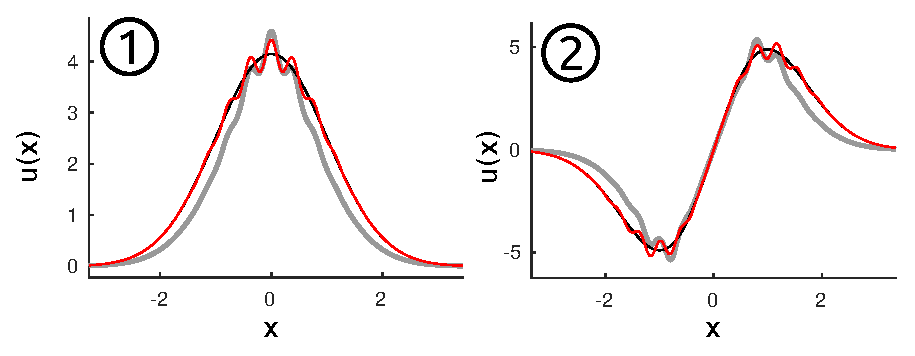
\includegraphics[width=0.9\textwidth]{Fig_5.eps}%\\
%    \includegraphics[width=0.8\textwidth]{nonlinear.eps}
\caption{Profiles of LMs, for $P(x)=\cos \left( 16x\right) $. (1) Branch $%
\Gamma _{0}$, $\protect\mu =0$ ($\Delta \protect\mu =1$). (2) Branch $\Gamma
_{1}$, $\protect\mu =1$ ($\Delta \protect\mu =2$). Gray line: the numerical
solution, red line: approximation (\protect\ref{AsRel_u}), with $U(x)$
obtained by numerical solution of Eq. (\protect\ref{U}). Blue line:
approximation (\protect\ref{u_appr_main}). }
\label{Fig:Prof}
\end{figure}

Combining the obtained results with Eq. (\ref{AsRel_u}), one finally gets
\begin{equation}
u(x)\approx \left( \frac{2{\mathcal{H}}_{n}^{(2)}\Delta \mu }{3{\mathcal{H}}%
_{n}^{(6)}}\right) ^{1/4}\sqrt{\Omega }H_{n}(x)e^{-x^{2}/2}+\left( \frac{2{%
\mathcal{H}}_{n}^{(2)}\Delta \mu }{3{\mathcal{H}}_{n}^{(6)}}\right) ^{3/4}%
\frac{\sigma _{1}}{\sqrt{\Omega }}H_{n}^{3}(x)e^{-3x^{2}/2}\cos \left(
\Omega x\right) .  \label{u_appr_main}
\end{equation}%
For the lowest branch $\Gamma _{0}$ Eq. (\ref{u_appr_main}) yields
\begin{equation}
u(x)\approx \left( \frac{2\Delta \mu }{\sqrt{3}}\right) ^{1/4}\sqrt{\Omega }%
e^{-x^{2}/2}+\left( \frac{2\Delta \mu }{\sqrt{3}}\right) ^{3/4}\frac{\sigma
_{1}}{\sqrt{\Omega }}e^{-3x^{2}/2}\cos \left( \Omega x\right) .
\end{equation}%
For the next branch, $\Gamma _{1}$, one obtains
\begin{equation}
u(x)\approx \left( \frac{216\Delta \mu }{15\sqrt{3}}\right) ^{1/4}\sqrt{%
\Omega }xe^{-x^{2}/2}+\left( \frac{216\Delta \mu }{15\sqrt{3}}\right) ^{3/4}%
\frac{\sigma _{1}}{\sqrt{\Omega }}x^{3}e^{-3x^{2}/2}\cos \left( \Omega
x\right) .
\end{equation}%
The comparison between the numerical solution and approximations (\ref%
{AsRel_u}) and (\ref{u_appr_main}) is illustrated by the Fig.~\ref{Fig:Prof}%
, for $\Omega =16$. The figure shows that approximation (\ref{AsRel_u})
describes the numerical solution very well. Approximation (\ref{u_appr_main}%
) is good too, even if $\Delta \mu $ is not small (compare grey and blue
lines in Fig.~\ref{Fig:Prof}, where $\Delta \mu =1$ and $2$ in the left and
right panels, respectively).

\subsubsection{Stability of localized modes}

\label{Gamma_stab}

In the small-amplitude limit, the stability of LMs is determined by
eigenvalues of matrix $\tilde{M}_{n}$, see Sect.~\ref{SmAmpl}. Using Maple,
one can compute these eigenvalues with any necessary accuracy. The results
for two modulation frequencies ($\Omega =8$ and $16$) are summarized in
Tables~\ref{T4}-\ref{T5}. In these tables, $n$ is the index of branch $%
\Gamma _{n}$ (for instance, $n=2$ means that branch $\Gamma _{2}$, which
starts from $\tilde{\mu}_{2}=2\cdot 2+1=5$, is under consideration), while $%
k $, running from $0$ to $n-1$, enumerates double eigenvalues $\tilde{\Lambda%
}_{k}=4(n-k)^{2}$. Each cell with $n>k$ contains either letter
``C" or two real numbers. These numbers
are the real eigenvalues $\gamma _{1,2}$ of the matrix $\tilde{M}_{n}$,
whereas ``C" means that both eigenvalues
of $\tilde{M}_{n}$ are complex. Dashes imply that the respective eigenvalues
do not exist. {\LARGE [I have added this statement - OK?]}

\begin{table}[tbp]
%[h]
\begin{tabular}{ccccccccccc}
& \phantom{111} & $n=1$ &  & $n=2$ &  & $n=3$ &  & $n=4$ &  & $n=5$ \\ \hline
$k=0$ &  & $%
\begin{array}{c}
0.132 \\
-0.028%
\end{array}%
$ &  & $%
\begin{array}{c}
-0.012 \\
0.203%
\end{array}%
$ &  & C &  & $%
\begin{array}{c}
0.424 \\
-0.828%
\end{array}%
$ &  & $%
\begin{array}{c}
-0.845 \\
-0.660%
\end{array}%
$ \\ \hline
$k=1$ &  & -- &  & $%
\begin{array}{c}
-0.176 \\
0.159%
\end{array}%
$ &  & $%
\begin{array}{c}
0.432 \\
-0.190%
\end{array}%
$ &  & $%
\begin{array}{c}
-0.486 \\
0.048%
\end{array}%
$ &  & $%
\begin{array}{c}
0.356 \\
0.944%
\end{array}%
$ \\ \hline
$k=2$ &  & -- &  & -- &  & $%
\begin{array}{c}
-0.068 \\
-0.132%
\end{array}%
$ &  & $%
\begin{array}{c}
-0.206 \\
0.196%
\end{array}%
$ &  & $%
\begin{array}{c}
0.531 \\
-0.600%
\end{array}%
$ \\ \hline
$k=3$ &  & -- &  & -- &  & -- &  & C &  & $%
\begin{array}{c}
0.166 \\
-0.122%
\end{array}%
$ \\ \hline
$k=4$ &  & -- &  & -- &  & -- &  & -- &  & C \\ \hline
\end{tabular}%
\caption{Eigenvalues of matrix $\tilde{M}$,\ in the case of $P(x)=\cos
\left( 8x\right) $. Here $n$ is the index of branch $\Gamma _{n}$, and $k$
enumerates double eigenvalues $\tilde{\Lambda}_{k}=4(n-k)^{2}$. Each cell
with $n>k$ contains either letter ``C" or
two real numbers. These numbers are real eigenvalues $\protect\gamma _{1,2}$
of matrix $\tilde{M}_{n}$, whereas letter ``C" means that eigenvalues 
of $\tilde{M}_{n}$ are complex.}
\label{T4}
\end{table}

\begin{table}[tbp]
%[h]
\begin{tabular}{ccccccccccc}
& \phantom{111} & $n=1$ &  & $n=2$ &  & $n=3$ &  & $n=4$ &  & $n=5$ \\ \hline
$k=0$ &  & $%
\begin{array}{c}
-2.0\cdot 10^{-11} \\
5.7\cdot 10^{-10}%
\end{array}%
$ &  & $%
\begin{array}{c}
-7.6\cdot 10^{-9} \\
-9.2\cdot 10^{-7}%
\end{array}%
$ &  & $%
\begin{array}{c}
-8.7\cdot 10^{-7} \\
2.2\cdot 10^{-4}%
\end{array}%
$ &  & $%
\begin{array}{c}
-4.0\cdot 10^{-5} \\
-1.2\cdot 10^{-2}%
\end{array}%
$ &  & $%
\begin{array}{c}
-9.5\cdot 10^{-4} \\
1.5\cdot 10^{-1}%
\end{array}%
$ \\ \hline
$k=1$ &  & -- &  & $%
\begin{array}{c}
-4.2\cdot 10^{-9} \\
7.3\cdot 10^{-8}%
\end{array}%
$ &  & $%
\begin{array}{c}
-5.8\cdot 10^{-7} \\
-3.6\cdot 10^{-5}%
\end{array}%
$ &  & $%
\begin{array}{c}
-3.0\cdot 10^{-5} \\
3.3\cdot 10^{-3}%
\end{array}%
$ &  & $%
\begin{array}{c}
-7.6\cdot 10^{-4} \\
-6.8\cdot 10^{-2}%
\end{array}%
$ \\ \hline
$k=2$ &  & -- &  & -- &  & $%
\begin{array}{c}
-3.4\cdot 10^{-7} \\
3.9\cdot 10^{-6}%
\end{array}%
$ &  & $%
\begin{array}{c}
-2.0\cdot 10^{-5} \\
-6.8\cdot 10^{-4}%
\end{array}%
$ &  & $%
\begin{array}{c}
-5.7\cdot 10^{-4} \\
2.6\cdot 10^{-2}%
\end{array}%
$ \\ \hline
$k=3$ &  & -- &  & -- &  & -- &  & $%
\begin{array}{c}
-1.3\cdot 10^{-5} \\
1.0\cdot 10^{-4}%
\end{array}%
$ &  & $%
\begin{array}{c}
-3.6\cdot 10^{-4} \\
-6.8\cdot 10^{-3}%
\end{array}%
$ \\ \hline
$k=4$ &  & -- &  & -- &  & -- &  & -- &  & $%
\begin{array}{c}
-2.7\cdot 10^{-4} \\
1.5\cdot 10^{-3}%
\end{array}%
$ \\ \hline
\end{tabular}%
\caption{Eigenvalues of matrix $\tilde{M}_{n}$ for $P(x)=\cos \left(
16x\right) $. The notation is the same as in Table \protect\ref{T4}.}
\label{T5}
\end{table}

To be specific, let us describe in detail branch $\Gamma _{2}$ in the case
of $P(x)=\cos \left( 8x\right) $, the branch $\Gamma _{2}$ (i.e., $n=2$ in
Table~\ref{T4}). In this case, there are two double eigenvalues in the
spectrum, $\tilde{\Lambda}_{0}=16$ and $\tilde{\Lambda}_{1}=4$. According to
Table~\ref{T4} and Eq. (\ref{Lambda_12_as}), they split as
\begin{equation}
\Lambda _{0}^{(1)}=16-0.012\cdot \varepsilon ^{2}+\ldots ,\quad \Lambda
_{0}^{(2)}=16+0.203\cdot \varepsilon ^{2}\ldots ~
\end{equation}%
and
\begin{equation}
\Lambda _{1}^{(1)}=4-0.176\cdot \varepsilon ^{2}+\ldots ,\quad \Lambda
_{1}^{(2)}=4+0.159\cdot \varepsilon ^{2}\ldots ~,
\end{equation}%
hence the small-amplitude nonlinear LMs belonging to branch $\Gamma _{2}$
are stable in this case. The situation is different for $\Gamma _{3,4,5}$,
since for each of these branches the bifurcation of a complex-conjugate pair
occurs: for $n=3$ the eigenvalue $\tilde{\Lambda}_{0}=36$ splits into
complex eigenvalues,while for $n=4$ and $n=5$ this takes place for $\tilde{%
\Lambda}_{2}=4$. Therefore, for $\Omega =8$ the small-amplitude LMs are
stable in branches $\Gamma _{0}$, $\Gamma _{1}$ and $\Gamma _{2}$, but
unstable in $\Gamma _{3}$, $\Gamma _{4}$ and $\Gamma _{5}$. Table~\ref{T5}
is produced for $\Omega =18$, implying that the small-amplitude LMs are
stable for \textit{all} the branches, $\Gamma _{0,...,5}$.

To explain the different stability of small-amplitude LMs with different
spatial frequencies $\Omega $, we consider the behavior of eigenvalues of $%
\tilde{M}_{n}$ at $\Omega \rightarrow \infty $. Using explicit results given
by Eqs. (\ref{11})--(\ref{22}) and asymptotic relation (\ref{AsGauss}), we
obtain %\begin{align}
%\la M_n\tilde u_k,\tilde u_k\ra&=\frac{8(n-k)}{\pi 2^{(n+k)}n!k!}\int_{-\infty}^\infty
%P(x)H_n^2(x)H_k^2(x)e^{-2x^2}~dx-\\[2mm] &- \frac{4(n-k)}{\pi
%2^{2n}(n!)^2}\int_{-\infty}^\infty P(x)H_n^4(x)e^{-2x^2}~dx\sim\\[2mm]
%&\sim -\frac{2\sqrt{2}(n-k)\Omega^{4n}}{2^{6n}\cdot(n!)^2 \sqrt{\pi} %}e^{-\Omega^2/8}=O(\Omega^{4n}e^{-\Omega^2/8}),
%\end{align}
%(the contribution of the first term in the right hand side of the last formula is of order $\sim \Omega^{2(n+k)} e^{-\Omega^2/8}$ that is small when compared with the second term).
%For the diagonal terms one has
%\begin{align}
%<M_n\tilde u_k,\tilde u_{2n-k}>&=-<M_n\tilde u_{2n-k},\tilde u_k>=\\[2mm]
%&=\frac{4(n-k)}{\pi 2^{2n}n!\sqrt{k!(2n-k)!}}\int_{-\infty}^\infty
%P(x)H_n^2(x)H_{2n-k}(x)H_k(x)e^{-2x^2}~dx\sim\\[2mm]
%&\sim\frac{2\sqrt{2}(n-k)\Omega^{4n}}{2^{6n}n!\sqrt{k!(2n-k)!} \sqrt{\pi} %}e^{-\Omega^2/8}=O(\Omega^{4n}e^{-\Omega^2/8}).
%\end{align}
%The asymptotics of the last entry is
%\begin{align}
%<M_n\tilde u_{2n-k},\tilde u_{2n-k}>&=-\frac{8(n-k)}{\pi 2^{(3n-k)}n!(2n-k)!}\int_{-\infty}^\infty
%P(x)H_n^2(x)H_{2n-k}^2(x)e^{-2x^2}~dx +\\[2mm]
%&\phantom{=}+ \frac{4(n-k)}{\pi
%2^{2n}(n!)^2}\int_{-\infty}^\infty P(x)H_n^4(x)e^{-2x^2}~dx\sim\\[2mm]
%&\sim-\frac{4\sqrt{2}(n-k)\Omega^{2(3n-k)}}{\sqrt{\pi}2^{3(3n-k)}n!(2n-k)!}
%e^{-\Omega^2/8}=O(\Omega^{2(3n-k)}e^{-\Omega^2/8}).
%\end{align}
%(again, due to (\ref{AsGauss}) the contribution of the first term in the sum dominates).
\begin{align}
\langle M_{n}\tilde{u}_{k},\tilde{u}_{k}\rangle & \sim -\frac{2\sqrt{2}%
(n-k)\Omega ^{4n}}{2^{6n}\cdot (n!)^{2}\sqrt{\pi }}e^{-\Omega ^{2}/8}, \\%
[2mm]
\langle M_{n}\tilde{u}_{k},\tilde{u}_{2n-k}\rangle & =-\langle M_{n}\tilde{u}%
_{2n-k},\tilde{u}_{k}\rangle \sim \frac{2\sqrt{2}(n-k)\Omega ^{4n}}{2^{6n}n!%
\sqrt{k!(2n-k)!}\sqrt{\pi }}e^{-\Omega ^{2}/8}, \\
\langle M_{n}\tilde{u}_{2n-k},\tilde{u}_{2n-k}\rangle & \sim -\frac{4\sqrt{2}%
(n-k)\Omega ^{2(3n-k)}}{\sqrt{\pi }2^{3(3n-k)}n!(2n-k)!}e^{-\Omega ^{2}/8}.
\end{align}%
These relations imply that
\begin{equation}
\tilde{M}_{n}=\left(
\begin{array}{cc}
O(\Omega ^{4n}e^{-\Omega ^{2}/8}) & O(\Omega ^{4n}e^{-\Omega ^{2}/8}) \\%
[2mm]
O(\Omega ^{4n}e^{-\Omega ^{2}/8}) & O(\Omega ^{2(3n-k)}e^{-\Omega ^{2}/8})%
\end{array}%
\right) ,\quad \Omega \rightarrow \infty
\end{equation}%
All elements of matrix $\tilde{M}_{n}$ are of the same order, except for the
one in the right lower corner which is of greater order due to $n>k$. This
means that, for\textit{\ }$\Omega $\textit{\ }large enough, eigenvalues of $%
\tilde{M}_{n}$\textit{\ }are real, hence the nonlinear LMs from branch $%
\Gamma _{n}$ for arbitrary $n$ are stable, at least in the small- amplitude
limit. This explains the difference between the results displayed in Tables~%
\ref{T4} and \ref{T5}: the increase of the spatial frequency from $\Omega =8$
to $\Omega =16$ results in stabilization of some small-amplitude LMs which
were originally unstable.
% from  is ``not enough large'' and Table \ref{T4} contains complex eigenvalues that implies the instability of the NLM.

Rigorously speaking, the results for the linear stability of the
small-amplitude LMs are asymptotic, and, while moving along branch $\Gamma
_{n}$ to the region of moderate or large amplitudes, the nonlinear LMs may
change the stability.
%The typical scenario for transition from stability to instability corresponds to the  collision of two reals eigenvalues with ensuing  bifurcations of a complex-conjugate pair.
To illustrate the persistence of the asymptotic predictions for the
(in)stability of the nonlinear LMs, in Fig.~\ref{CollEig} we plot
numerically obtained dependencies of eigenvalues $\lambda $ on $\mu $ for
branches $\Gamma _{0,1,2,3}$ in the case of $P(x)=\cos \left( 16x\right) $.
Each shown branch is stable near the point of its emergence, losing
stability at some threshold value of $\mu $ (which is different for
different branches).

\begin{figure}[tbp]
\includegraphics[width=0.6\textwidth]{Fig_Eigens_1.eps}%\\
%    \includegraphics[width=0.8\textwidth]{nonlinear.eps}
\caption{The evolution of eigenvalues of (\protect\ref{EigProb}) as $\protect%
\mu $ varies, for $P(x)=\cos \left( 16x\right) $. Only eigenvalues with $%
\mathrm{Im}~\protect\lambda \geq 0$ are shown. Solid line: pure imaginary
eigenvalues corresponding to stable LMs; dashed line: eigenvalues with a
nonzero real part. (1) Branch $\Gamma _{0}$. No double eigenvalues exist at $%
\protect\mu =1$, all the eigenvalues being pure imaginary and simple, until
the collision at $\mu\approx -1.049$. After the collision a
pair of real eigenvalues emerges. (2) Branch $\Gamma _{1}$. At $\protect\mu %
=3$ there exists one double eigenvalue, $\protect\lambda =2i$. According to
the prediction of the asymptotic analysis, it splits into a pair of pure
imaginary simple eigenvalues. The collision of eigenvalues occurs at
$\mu\approx 1.372$, and a pair of eigenvalues with nonzero
real parts emerges. (3) Branch $\Gamma _{2}$. At $\protect\mu =5$, there
exists two pairs of double eigenvalues, $\protect\lambda =2i$ and $\protect%
\lambda =4i$. Both of them split into pairs of pure imaginary eigenvalues.
The former pair collides again at $\mu\approx 4.801$ and
transforms into a pair of complex eigenvalues with nonzero real parts. At
$\mu\approx 3.519$ , another collision of eigenvalues
occurs. (4) Branch $\Gamma _{3}$. At $\protect\mu =7$, there exist three
pairs of double eigenvalues. The first collision of pure imaginary
eigenvalues takes place at $\mu\approx 5.571$, then two more
collisions occur. They all result in eigenvalues with nonzero real parts.}
\label{CollEig}
\end{figure}

Numerically generated $N(\mu )$ curves for $\Omega =8$, $\Omega =12$, and $%
\Omega =16$ are plotted in Fig.~\ref{Fig_ZM_branches}. It follows from these
plots that branch $\Gamma _{0}$ is the ``most
stable" one for all the three values of $\Omega $. One
also notices that, for the greatest value of $\Omega $ (i.e., $\Omega =16$)
there exists a ``stability window" in a
vicinity of the bifurcations for all branches $\Gamma _{0,1,2,3}$, in
agreement with the asymptotic results presented above.

Numerical study of the temporal evolution of LMs in the framework of
time-dependent GPE~(\ref{1D_GP_12}) confirms the predictions of the
linear-stability analysis, see Fig.~\ref{Fig_Comp_NZM}(2a,b).
% We observe several ways for breaking down of unstable NLMs.
%An example of
As an example of a distinctive pattern of dynamical behavior of unstable
modes, in Fig.~\ref{Fig_Comp_NZM}(2b) we display its transformation into a
pulsating object localized over one period of the lattice pseudopotential.

\begin{figure}[tbp]
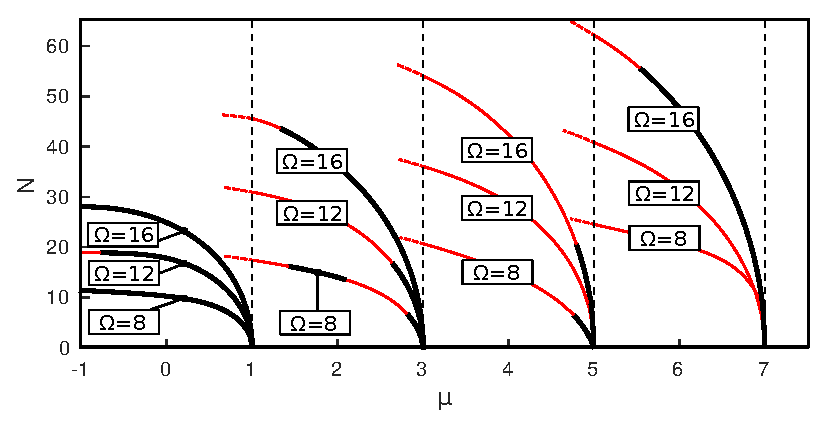
\includegraphics[width=0.8\textwidth]{Fig_3_v2_extended.eps}%\\
%    \includegraphics[width=0.8\textwidth]{nonlinear.eps}
\caption{$N(\protect\mu )$ curves for $P(x)=\cos \left( \Omega x\right) $, $%
\Omega =8,12,16$. Branches $\Gamma _{0,1,2,3}$ are presented. Black bold
(red thin) lines correspond to stable (unstable) LMs.}
\label{Fig_ZM_branches}
\end{figure}

%\subsubsection{The evolution of NLM}\label{Evol_ZM}

\begin{figure}[tbp]
\includegraphics[width=0.8\textwidth]{Fig_7_ZM_1.eps}%\\
%    \includegraphics[width=0.8\textwidth]{nonlinear.eps}
\caption{The case of $P(x)=\cos \left( 16x\right) $. (1a): The evolution of
a stable nonlinear mode belonging to branch $\Gamma _{1}$, with $\protect\mu %
=2$. (1b): the spectrum of eigenvalues $\protect\lambda $ produced by
numerical solution of Eq. (\protect\ref{EigProb}) associated with this mode.
(2a): The evolution of an unstable mode belonging to branch $\Gamma _{1}$,
with $\protect\mu =0$; (2b) the corresponding spectrum. }
\label{Fig_Comp_ZM}
\end{figure}

\section{Conclusion}

\label{Concl}

In the paper, we have systematically studied nonlinear LMs (localized modes)
of the one-dimensional Gross-Pitaevskii/nonlinear Schr\"{o}dinger equation
with the HO (harmonic-oscillator) trapping potential $V(x)$ and nonlinear
lattice pseudopotential $P(x)$, which is an periodic function oscillating
with spatial frequency $\Omega $. %From the physical viewpoint,
The equation describes a cigar-shaped cloud of BEC confined by the magnetic
trap and manipulated by the optically-induced Feshbach resonance with the
periodically modulated local strength. The model is characterized by the
interplay between two spatial scales: the characteristic size of the HO trap
and the period of the nonlinear lattice pseudopotential. This factor
essentially enriches the variety of nonlinear modes in this model, in
comparison with the well-studied case of the spatially uniform nonlinearity.
We have obtained analytical results of the shape of nonlinear LMs and on
their stability, in the limits of small-amplitude solutions and rapidly
oscillating pseudopotential. The validity and persistence of the asymptotic
predictions has been corroborated by systematically presented numerical
findings.

%. The interplay of the two scales opens new perspectives for creation of novel stable matter waves as well as their handling. The paper is aimed to found NLM in this model and to compare the results with the ones for the case $P(x)={\rm const}$ (called above {\it the nonlinear harmonic oscillator}) that was analysed in many studies.

To conclude the paper, it is relevant, once again, the highlight main
results of the work. %
%We present general pictures of NLM branches for various relations between the characteristic sizes. When the scales are comparable, we employ numerical methods. The computations are based on the algorithm of the paper \cite{AZ07} that allows to find all the NLM in the given range of parameters. Also we used asymptotic methods, if the period of the pseudopotential is small compared with the characteristic size of the parabolic trap.
It was found that there exist two types of branches of LMs, \textit{viz}.,
ones with and without linear counterpart. This is especially interesting in
view of the fact that no modes without linear counterpart exists in the
model with the uniform nonlinearity. However, all these ``exotic" 
nonlinear modes, disconnected from the linear limit, are unstable.
As concerns nonlinear LMs bifurcating from eigenstates of the underlying
linear problem, their properties are essentially different depending on the
presence of the dc term (nonzero mean value) in the periodic
pseudopotential. In the mean is nonzero, then properties of nonlinear modes
in a rapidly oscillating pseudopotential may be approximated using solutions
for the standard HO model with constant nonlinearity. However, the reduction
to the standard model with constant nonlinearity does not work for the
system in a rapidly oscillating pseudopotential without the dc term. Most
interestingly, in this case we have found that the rapidly oscillating
pseudopotential can stabilize small-amplitude LMs belonging to higher
families (excited states, which are unstable in the model including the dc
term). Specifically, for any given branch with index $n$, there exists a
threshold values of the spatial frequency, $\Omega _{n}$, such that the
small-amplitude solutions belonging to this branch are stable for $\Omega
>\Omega _{n}$.

As a continuation of this work, it may be interesting to extend the analysis
to the case of the interplay of the spatially periodic pseudopotential with
the expulsive (anti-HO) potential. A more challenging possibility is to
consider a two-dimensional model featuring the combination of an isotropic
HO trapping potential and two-dimensional lattice quasipotential.
%Using our asymptotic results, the threshold values $\Omega_n$ can be obtained explicitly.\textcolor{red}{[.. Dima, the last sentence: what do you mean?..]}
{\LARGE \ [A general request: in the caption of each figure, please write if
it corresponds to the model with or without the dc term; otherwise, it is
difficult to read the figures.]}

% Any family of NLM with linear counterpart branches off from zero solution and therefore includes NLMs of arbitrarily small amplitude. Contrarily, the families of NLM without linear counterpart have no small amplitude limit. No families without linear counterpart exist in the case $P(x)={\rm const}$, therefore their existence is caused by variable coefficient $P(x)$.

%We consider separately the two cases: the first, when $P(x)$ has nonzero mean and the second, when $P(x)$ has nonzero mean. In the first case, the NLM with linear counterpart approaches the corresponding modes of nonlinear harmonic oscillator, when the period of $P(x)$ tends to zero. In the second case, we show that high frequency oscillations of $P(x)$ can stabilize small amplitude NLM corresponding to higher order branches.

\acknowledgements

The research of G.L.A., M.E.L. and D.A.Z. was supported by Russian Science
Foundation (Grant No. 17-11-01004). The work of B.A.M. is supported, in
part, by the joint program in physics between NSF and Binational (US-Israel)
Science Foundation through project No. 2015616, and by the Israel Science
Foundation through Grant No. 1286/17

\begin{thebibliography}{99}
\bibitem{AEMWC95} M. H. Anderson, J. R. Ensher, M. R. Matthews, C. E.
Wieman, and E. A. Cornell, Observation of Bose-Einstein condensation in a
dilute atomic vapor, Science \textbf{269}, 198 (1995).

\bibitem{DMADDKK95} K. B. Davis, M.-O. Mewes, M. R. Andrews, N. J. van
Druten, D. S. Durfee, D. M. Kurn, and W. Ketterle, Bose-Einstein
condensation in a gas of sodium atoms, Phys. Rev. Lett. \textbf{75}, 3969
(1995).

\bibitem{BSTH95} C. C. Bradley, C. A. Sackett, J. J. Tollett, and R. G.
Hulet, Evidence of Bose-Einstein condensation in an atomic gas with
attractive interactions, Phys. Rev. Lett. \textbf{75}, 1687 (1995).

\bibitem{Romanian} V. S. Bagnato, D. J. Frantzeskakis, P. G. Kevrekidis, B.
A. Malomed, and D. Mihalache, Bose-Einstein condensation: Twenty years
after, Rom. Rep. Phys. \textbf{67}, 5-50 (2015).

\bibitem{I98} Inouye, S., M. R. Andrews, J. Stenger, H. J. Miesner, D. M.
Stamper- Kurn, and W. Ketterle, Observation of Feshbach resonances in a
Bose-Einstein condensate, Nature (London) \textbf{392}, 151, (1998).

\bibitem{TT04} Theis, M., G. Thalhammer, K. Winkler, M. Hellwig, G. Ruff, R.
Grimm, and J. H. Denschlag, Tuning the scattering length with an optically
induced Feshbach resonance, Phys. Rev. Lett. \textbf{93}, 123001 (2004).

\bibitem{KGJ06} T. Kohler, K. Goral and P. S. Julienne, Production of cold
molecules via magnetically tunable Feshbach resonances, Rev. Mod. Phys.
\textbf{78}, 1311 (2006).

\bibitem{Hannaford} S. Ghanbari, T. D. Kieu, A. Sidorov, and P. Hannaford,
Permanent magnetic lattices for ultracold atoms and quantum degenerate
gases, J. Phys. B: At. Mol. Opt. Phys. \textbf{39}, 847-860 (2006).

\bibitem{Japan} R. Yamazaki, S. Taie, and S. Sugawa, and Y. Takahashi,
Submicron spatial modulation of an interatomic interaction in a
Bose-Einstein condensate, Phys. Rev. Lett. \textbf{105}, 050405 (2010).

\bibitem{Cs} L. W. Clark, L.-C. Ha, C.-Y. Xu, and C. Chin, Quantum dynamics
with spatiotemporal control of interactions in a stable Bose-Einstein
condensate, Phys. Rev. Lett. \textbf{115}, 155301 (2015).

\bibitem{HS} H. Sakaguchi and B. A. Malomed, Solitons in combined linear and
nonlinear lattice potentials, Phys. Rev. A \textbf{81}, 013624 (2010).

\bibitem{Pet} C. J. Pethick and H. Smith, \textit{Bose-Einstein Condensation
in Dilute Gases} (Cambridge University Press: Cambridge, 2002).

\bibitem{Pit} L. P. Pitaevskii and A. Stringari, \textit{Bose-Einstein
Condensation} (Clarendon Press: Oxford, 2003).

\bibitem{Salasnich} L. Salasnich, A. Parola, and L. Reatto, Effective wave
equations for the dynamics of cigar-shaped and disk-shaped Bose
condensates , Phys. Rev. A \textbf{65}, 043614 (2002).

\bibitem{Delgado} A. Mu\~{n}oz Mateo and V. Delgado, Effective mean-field
equations for cigar-shaped and disk-shaped Bose-Einstein
condensates, Phys. Rev. A \textbf{77}, 013617 (2008).

\bibitem{pseudo} W. A. Harrison, \textit{Pseudopotentials in the Theory of
Metals }(Benjamin: New York, 1966).

\bibitem{ZAKP07} D. A. Zezyulin, G. L. Alfimov, V. V. Konotop and V. M. P%
\'{e}rez-Garc\'{\i}a, Control of nonlinear modes by scattering-length
management in Bose-Einstein condensates, Phys. Rev. A \textbf{76}, 013621
(2007)

\bibitem{TAM16} F. Tsitoura, Z. A. Anastassi, J. L. Marzuola, P. G.
Kevrekidis, and D. J. Frantzeskakis, Dark solitons near potential and
nonlinearity steps, Phys. Rev. A \textbf{94}, 063612 (2016).

\bibitem{RKP08} A. S. Rodrigues, P. G. Kevrekidis, M. A. Porter, D. J.
Frantzeskakis, P. Schmelcher, and A. R. Bishop, Matter-wave solitons with a
periodic, piecewise-constant scattering length, Phys. Rev. A 78, 013611
(2008).

\bibitem{WLK13} C. Wang, K. J. H. Law, P. G. Kevrekidis, and M. A. Porter,
Dark solitary waves in a class of collisionally inhomogeneous Bose-Einstein
condensates, Phys. Rev. A \textbf{87}, 023621 (2013)

\bibitem{SM05} H. Sakaguchi, B. A. Malomed, Matter-wave solitons in
nonlinear optical lattices, Phys. Rev. E 72, 046610 (2005)

\bibitem{K17} P. G. Kevrekidis, R. Carretero-Gonz\'{a}lez, and D. J.
Frantzeskakis, Stability of single and multiple matter-wave dark solitons in
collisionally inhomogeneous Bose Einstein condensates, Intern. J. Mod. Phys.
B \textbf{31}, 1742013 (2017).

\bibitem{OL} O. Morsch and M. Oberthaler, Dynamics of Bose-Einstein
condensates in optical lattices, Rev. Mod. Phys. \textbf{78}, 179-215 (2006).

\bibitem{TSKF02} G. Theocharis, P. Schmelcher, P. G. Kevrekidis, and D. J.
Frantzeskakis,
%G. Theocharis,1,4 P. Schmelcher,1,2 P. G. Kevrekidis,3 and D. J. Frantzeskakis
Phys. Rev. \textbf{72}, 033614 (2005).

\bibitem{HY08} R. Hao, R, Yang, L. Li, and G. Zhou, Solutions for the
propagation of light in nonlinear optical media with spatially inhomogeneous
nonlinearities, Opt. Commun. \textbf{281}, 1256 (2008).

\bibitem{KMT11} Y. V. Kartashov, B. A. Malomed, and L. Torner, Solitons in
nonlinear lattices, Rev. Mod. Phys. \textbf{83}, 247-306 (2011).

\bibitem{Barcelona} O. V. Borovkova, Y. V. Kartashov, L. Torner, and B. A.
Malomed, Bright solitons from defocusing nonlinearities, Phys. Rev. E
\textbf{84}, 035602 (R) (2011).

\bibitem{C10} M. P. Coles, D. E. Pelinovsky, and P. G. Kevrekidis, Excited
states in the large density limit: a variational approach, Nonlinearity
\textbf{23}, 1753-1770 (2010).

\bibitem{PFK05} D. E. Pelinovsky, D. J. Frantzeskakis, and P. G. Kevrekidis,
Oscillations of dark solitons in trapped Bose-Einstein condensates, Phys.
Rev. E \textbf{72}, 016615 (2005).

\bibitem{DM15} N. Dror and B. A. Malomed, Solitons and vortices in nonlinear
potential wells, J. Opt. \textbf{18}, 014003 (2016).

\bibitem{AZ07} G. L. Alfimov and D. A. Zezyulin, Nonlinear modes for the
Gross-Pitaevskii equation -- a demonstrative computation approach,
Nonlinearity \textbf{20}, 2075-2092 (2007).

%\bibitem{BerShub}
%     F.A. Berezin and M.A. Shubin M A, {\it The Shr\"odinder equation}, Kluwer Academic  Publisher, 1991.
%\bibitem{Fedoryuk}
%     M.V. Fedoryuk {\it Asymptotic Analysis. Linear Ordinary Differential Equations}, Springer, 1993
%\bibitem{inWasov}
%     M.V. Fedoryuk, Asymptotics of solutions of linear differential
%     equations of the second order in complex domain, Addendum 1 to russian translation of: Wasov W 1968 {\it Asymptotic Expansions for Ordinary Differential Equations}. Moscow: Mir, 1968, (in Russian).

\bibitem{AKS02} G. L. Alfimov, V. V. Konotop and M. Salerno, Matter solitons
in Bose-Einstein Condensates with optical lattices, Europhys. Lett. \textbf{%
58}, 7-13 (2002).

\bibitem{JYang} J. Yang, \textit{Nonlinear Waves in Integrable and
Nonintegrable Systems} (Society for Industrial and Applied Mathematics:
Philadelphia, 2010).

\bibitem{AMP} R. D'Agosta, B. A. Malomed and C. Presilla, Laser Phys.
\textbf{12}, 37 (2002).

\bibitem{AP} R. D'Agosta and C. Presilla 2002 Phys. Rev. A \textbf{65},
043609.

\bibitem{Zeng} J. Zeng and B. A. Malomed, Localized dark solitons and
vortices in defocusing media with spatially inhomogeneous nonlinearity,
Phys. Rev. E \textbf{95}, 052214 (2017).

\bibitem{E95} M. Edwards and K. Burnett,
% Numerical Solution of the Nonlinear Schrödinger Equation for Small Samples of Trapped Neutral Atoms.
Phys. Rev. A \textbf{51}, 1382-1386 (1995).

\bibitem{K99} M. Kunze, T. K\"upper, V. K. Mezentsev, E. G. Shapiro, S.
Turitsyn, % Nonlinear Solitary Waves with Gaussian Tails.
Physica D \textbf{128}, 273--295 (1999).

\bibitem{G99} A. Gammal, T. Frederico, and L. Tomio,
%Improved numerical approach for the time-independent Gross-Pitaevskii nonlinear Schro¨dinger equation
Phys. Rev. E \textbf{60}, 2421 (1999).

\bibitem{KAT01} Yu. S. Kivshar, T. J. Alexander and S. K. Turitsyn, Phys.
Lett. A \textbf{278}, 225 (2001).

\bibitem{C01} L. D. Carr, J. N. Kutz, and W. P. Reinhardt, Phys. Rev. E
\textbf{63}, 066604 (2001).

\bibitem{YYB02} V. I. Yukalov, E. P. Yukalova, and V. S. Bagnato, Phys. Rev.
A \textbf{66}, 043602 (2002).

\bibitem{KK03} V. V. Konotop and P. G. Kevrekidis,
%V.V. Konotop1 and P. G. Kevrekidis
Phys. Rev. Lett. \textbf{91}, 230402 (2003).

\bibitem{ZAKP08} D. A. Zezyulin, G. L. Alfimov, V. V. Konotop, V. M. P\'{e}%
rez-Garc\'{\i}a, Stability of excited states of a Bose-Einstein condensate
in an anharmonic trap, Phys. Rev. A \textbf{78}, 013606 (2008).

\bibitem{KKRF05} P. G. Kevrekidis, V. V. Konotop, A. Rodrigues, and D. J.
Frantzeskakis, Dynamic generation of matter solitons from linear states via
time-dependent scattering lengths, J. Phys. B: At. Mol. Opt. Phys. \textbf{38%
}, 1173-1178 (2005).

\bibitem{ZK16} D. A. Zezyulin and V. V. Konotop, Small-amplitude nonlinear
modes under the combined effect of the parabolic potential, nonlocality and $%
\mathcal{PT}$ Symmetry, Symmetry \textbf{8}, 72 (2016).

\bibitem{Fatkhulla} F. Kh. Abdullaev, J. G. Caputo, R. A. Kraenkel, and B.
A. Malomed, Controlling collapse in Bose-Einstein condensation by temporal
modulation of the scattering length, Phys. Rev. A \textbf{67}, 013605 (2003).

\bibitem{TP} V. A. Trofimov and N. V. Peskov, Comparison of
finite-difference schemes for the Gross-Pitaevskii equation, Mathematical
Modelling and Analysis \textbf{14}, 109 (2009).
\end{thebibliography}

\end{document}
